\documentclass[a4paper]{article}
\usepackage[top=1in,bottom=1in,left=1in,right=1in]{geometry}
\usepackage{enumitem}
\usepackage{mathtools}
\usepackage{graphicx}
\usepackage{float}
\usepackage{hyperref}
\usepackage{tabularx}
\usepackage{float}
\usepackage[table]{xcolor}

%opening
\title{Manual Penggunaan Mediklik}

\begin{document}

\maketitle
\section{Menu Awal}
\begin{figure}[H]
	\centering
	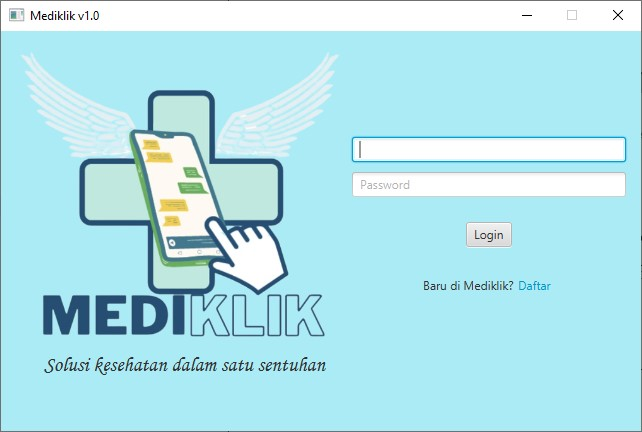
\includegraphics[width=0.5\textwidth]{imgs/mediklik_1.jpg}
\end{figure}
\par Ketika Anda membuka Mediklik, Anda akan disambut oleh menu awal. Anda dapat masuk log dengan akun yang sudah ada, atau membuat akun baru. Jika Anda mencoba memasukan nama pengguna atau password yang salah, maka program akam memperingati Anda.
\subsection{Registrasi}
\begin{figure}[H]
	\centering
	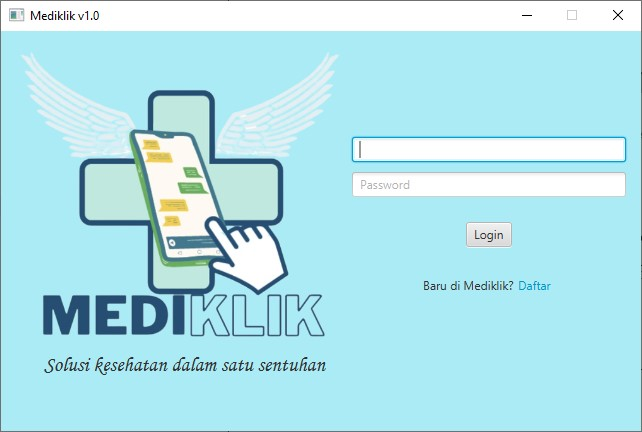
\includegraphics[width=0.5\textwidth]{imgs/mediklik_2.jpg}
\end{figure}
\par Di menu ini, Anda dapat membuat akun yang baru. Mediklik akan menanyakan username dan password anda. Jika username yang anda masukkan sudah digunakan oleh akun lain, maka program akan memperingati Anda. Setelah anda mendaftarkan akun Anda, maka Anda akan masuk log ke dalam menu utama.
\section{Item Browsing}
\begin{figure}[H]
	\centering
	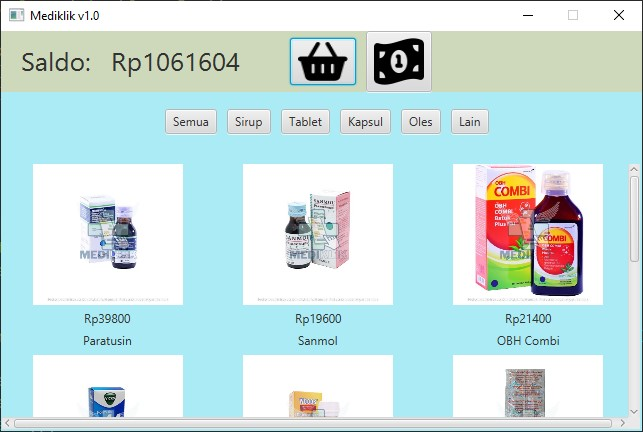
\includegraphics[width=0.5\textwidth]{imgs/mediklik_3.jpg}
\end{figure}
\par Di menu ini, Anda dapat mencari item yang Anda inginkan. Di bagian atas muncul saldo Anda, tombol keranjang, dan tombol top-up saldo. Di bawahnya anda dapat menyaring produk yang anda cari dengan memilih kategori tertentu. Jika anda menekan gambar, harga, atau nama dari suatu produk, maka Anda akan dibawa ke menu item tersebut.
\section{Menu Item}
\begin{figure}[H]
	\centering
	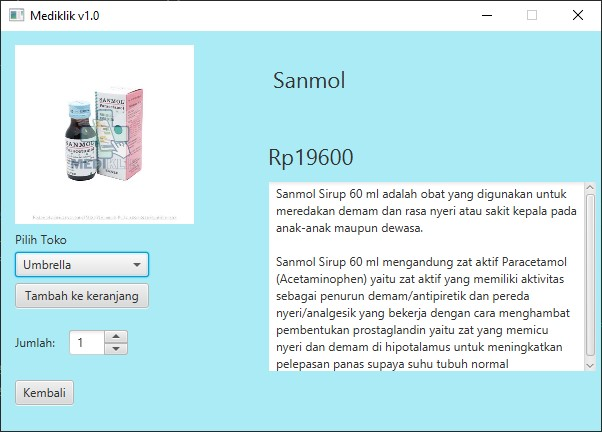
\includegraphics[width=0.5\textwidth]{imgs/mediklik_7.jpg}
\end{figure}
\par Di menu ini, anda dapat melihat detail dari suatu item. Anda dapat menambahkan item tersebut ke keranjang Anda dengan menekan tombol "Tambah ke keranjang".
\section{Keranjang}
\begin{figure}[H]
	\centering
	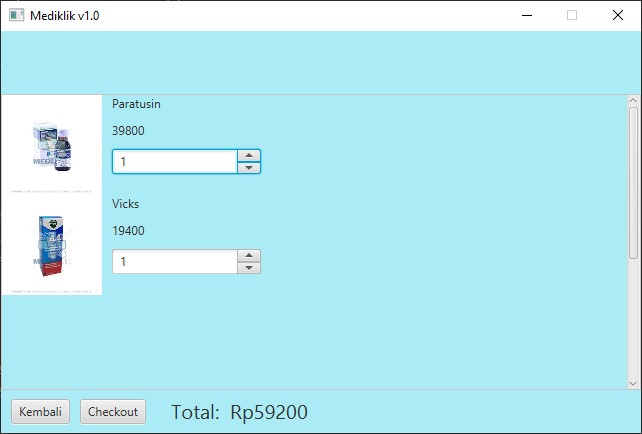
\includegraphics[width=0.5\textwidth]{imgs/mediklik_4.jpg}
\end{figure}
\par Di menu ini, Anda dapat melihat item yang sudah dimasukkan ke dalam keranjang Anda. Jika anda ingin melanjutkan pembelian, maka tekan tombol checkout untuk menuju menu checkout.
\section{Saldo}
\begin{figure}[H]
	\centering
	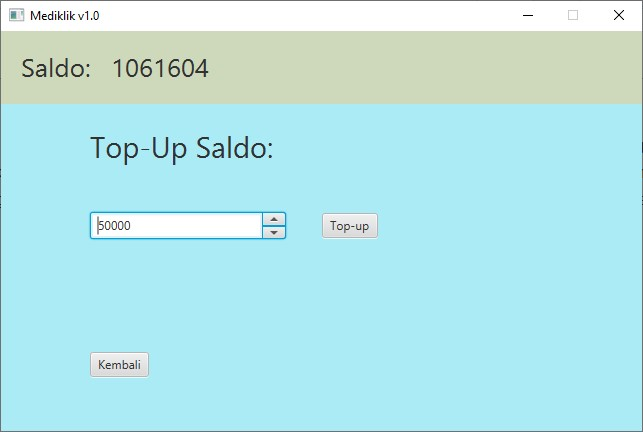
\includegraphics[width=0.5\textwidth]{imgs/mediklik_6.jpg}
\end{figure}
\par Di menu ini, Anda dapat melihat berapa saldo yang anda miliki. Anda juga bisa menambah saldo Anda dengan menggunakan menu yang tersedia.
\end{document}
